% homework/caffeine/caffeine.tex
% Year 7 - Science Models, Part 2: Challenge Homework. Why Is Mr Bowen Still
% Awake?
%
% EIGHT PAGES (two A4 sheets, double-sided). The first draft was 13 and the
% teacher called it "way too many pages". Keep it at eight.
%
% Goes home after Part 2 of the Models deck (content/y7-science/U03_models,
% slides 18-46). Every number the deck gave is kept: caffeine's half-life is
% 5 hours, a cup of coffee is about 100 mg, carbon-14's half-life is 5 700
% years, carbon dating works up to about 50 000 years.
%
% ONE SPINE. The deck's coffee was a made-up 100 mg at 7 a.m. This sheet starts
% from Mr Bowen's REAL day and ends with a real person the student knows:
%   Part A  Mr Bowen's real day in half-life steps. Two cold brews from
%           Jeremy's at 8 a.m. (200 mg each), a double-shot oat milk latte at
%           1 p.m. (2 x 60 mg), bed at 11 p.m. The times are 5 hours apart on
%           purpose, so the halving is exact: 400, 200 (+120) 320, 160, 80.
%           8 p.m. is OFF the grid, so it is read from the graph (about 121).
%   Part B  The hour-by-hour rule (x 0.87 every hour, + a drink when they
%           drink), because nobody at home drinks exactly every 5 hours.
%           0.87^5 = 0.498, so it IS the 5-hour half-life. B2 runs it from
%           1 p.m. to 8 p.m.: 160 at 6 p.m. (A2 says 160) and 121 at 8 p.m.
%           (the graph says about 120). Deck slide 43: when different methods
%           agree, scientists trust the answer.
%   Part C  THE MAIN TASK. Interview an adult at home, look up each drink,
%           build the hour-by-hour table and the graph, and estimate their
%           caffeine at bedtime. Ends with one limitation of the model.
%   Part D  Carbon dating: the halving chain, a museum table with three traps
%           (charcoal and cotton WERE alive; a stone axe never was; a T. rex is
%           too old), and what caffeine and carbon-14 have in common: top-ups,
%           then halving.
%
% Mr Bowen's numbers, hour by hour, rounded at every step (the key uses them):
%   8 400 | 9 348 | 10 303 | 11 264 | 12 230 | 1 200 +120 = 320 | 2 278 |
%   3 242 | 4 211 | 5 184 | 6 160 | 7 139 | 8 121 | 9 105 | 10 91 | 11 79
%
% Nothing untaught: x 0.87 and 3.3 x 20 are Unit 4 decimals, the mean of two
% numbers is HW 9, reading a scale is HW 8 Section F. Calculators are allowed.
% The 400 mg a day for adults is given on the page, not assumed.
%
% English only for now. If a French copy is wanted, follow hw09x: \fr lines,
% \FRENCH build, even page count.
%
% House style is shared: see homework/hw-style.tex. Method: the new-homework
% skill. Source is pure ASCII on purpose.
%
% Build:  pwsh .claude/skills/new-homework/scripts/build-hw.ps1 caffeine

\documentclass[12pt,a4paper]{article}

% -- Answer key switch -------------------------------------------------------
\newif\ifkey
\ifdefined\TEACHER\keytrue\else
  \keyfalse        % \keyfalse = student copy   |   \keytrue = teacher copy
\fi

% -- House style -------------------------------------------------------------
% homework/hw-style.tex
% Shared house style for every Year 7 homework packet. \input this from the
% packet file, right after \documentclass and the answer-key switch.
%
% Do not fork this file per packet. If a packet needs a different look, the
% question is whether every packet should have it.
%
% The choices here are deliberate and were arrived at by printing and looking:
%   * No solid dark banners. Every header is a light tint with a coloured spine
%     on the left, so colour reads clearly without flooding a school printer.
%   * No marks and no mark totals. These are practice, not exam papers.
%   * Lato at 12pt with open leading, plus mathastext so inline maths is Lato
%     too. Without mathastext every "-6 + 4" is Computer Modern serif and the
%     sheet looks half-typeset.
%   * Writing lines are spaced for Year 7 handwriting, not adult margin notes.
%   * Pages fill. \needspace is redefined below so a heading no longer drags
%     the page break up to itself, and every heading is glued to the box under
%     it. Packets built before 2026-09-30 were laid out under the old rules and
%     will reflow if rebuilt -- re-read every page if you rebuild one.
%
% Provides: \wlines \blank \tickbox \sep \qmk-free marks (none) \hwsection
% \qhead \expr, the workspace box, and the remember / wordhelp / activity /
% yourturn coloured boxes. Palette matches the lesson decks exactly.

% -- Packages ----------------------------------------------------------------
\usepackage[T1]{fontenc}
\usepackage[utf8]{inputenc}
\usepackage[default]{lato}
\usepackage[a4paper,top=1.7cm,bottom=1.7cm,left=2.0cm,right=2.0cm,headheight=15pt]{geometry}
\usepackage{amsmath,amssymb}
\usepackage{xcolor}
\usepackage[most]{tcolorbox}
\usepackage{enumitem}
\usepackage{tikz}
\usetikzlibrary{arrows.meta}
\usepackage{array}
\usepackage{tabularx}
\usepackage{fancyhdr}
\usepackage{multicol}
\usepackage{needspace}
\usepackage{graphicx}

% Make maths use Lato too. Without this, every "-6 + 4" on the page is set in
% Computer Modern serif and the sheet looks half-typeset. Must come last.
\usepackage[italic]{mathastext}

% -- \needspace, without the hole it used to leave ----------------------------
% needspace.sty writes "\vskip 0pt plus X \penalty-100" in front of every
% heading. A page that ends anywhere else is underfull with no stretch, so TeX
% scores it b=10000; a page that ends AT a heading gets that X of stretch and a
% finite badness, and wins. So any heading in roughly the bottom half of a page
% claimed the break, and the question under it moved over whole, leaving a hole
% the size of the question. \tracingpages showed it exactly (b=4531 at the
% heading, b=10000 at every later break) while building homework/q1rev, and it
% is where the half-empty pages in HW 1-8 came from.
% This keeps only the \penalty9999, which still refuses to put a heading in the
% last X of a page. Keeping a heading WITH the box under it is \nobreak's job
% now -- see \hwsection and \qhead below.
\makeatletter
\renewcommand{\needspace}[1]{\begingroup\setlength{\dimen@}{#1}%
  \vskip\dimen@\penalty9999\vskip-\dimen@\endgroup}
\makeatother

\linespread{1.06}\selectfont

% -- The Learner's Book palette (same hex values as the lesson decks) ---------
\definecolor{cbteal}{HTML}{0087A8}
\definecolor{cbpurple}{HTML}{5C2483}
\definecolor{cborange}{HTML}{C25E12}
\definecolor{cbgreen}{HTML}{4A8B23}
\definecolor{cbred}{HTML}{C8102E}
\definecolor{cbblue}{HTML}{1A5FA8}
\definecolor{rulegray}{HTML}{9AA5AD}

% -- Answer lines and blanks -------------------------------------------------
% \wlines{n} draws n ruled writing lines, spaced wide enough for Year 7
% handwriting rather than for an adult with a fine pen.
\makeatletter
\newcommand{\wlines}[1]{%
  \par\vspace{0.75em}%
  \@tempcnta=0\relax
  \@whilenum\@tempcnta<#1\do{%
    \hbox to \linewidth{\color{rulegray}\leaders\hrule height 0.5pt\hfill}%
    \vspace{1.5em}%
    \advance\@tempcnta by 1\relax}%
  \par\vspace{-0.8em}%
}
\makeatother

% \blank[width] is an inline gap to write a short answer in.
\newcommand{\blank}[1][2.6cm]{\underline{\hspace{#1}}}

% A boxed space for showing working.
\newtcolorbox{workspace}[1][3.4cm]{%
  colback=white, colframe=rulegray, boxrule=0.5pt, arc=5pt,
  height=#1, left=6pt, right=6pt, top=4pt, bottom=4pt,
  before skip=9pt, after skip=11pt}

% An empty tick box.
\newcommand{\tickbox}{\fbox{\rule{0pt}{1.15em}\rule{1.15em}{0pt}}}

% A middot separator.
\newcommand{\sep}{\,\textperiodcentered\,}

% -- Section and question headings -------------------------------------------
% Light tint plus a fat coloured spine on the left. No solid dark banner: the
% colour reads clearly but barely costs the printer anything.
% needspace keeps a heading out of the last few lines of a page. The \nobreak
% after it keeps it with whatever comes next: a remember or word-help box that
% does not fit takes its heading over with it, instead of leaving the heading
% alone at the foot of the page. (The old needspace did that by accident, and
% left a hole every time; see above.)
\newcommand{\hwsection}[2][cbteal]{%
  \needspace{8\baselineskip}%
  \par\vspace{13pt}%
  \noindent
  \begin{tcolorbox}[enhanced, nobeforeafter, width=\textwidth,
      colback=#1!7, colframe=#1!7, arc=5pt,
      borderline west={5pt}{0pt}{#1},
      left=14pt, right=10pt, top=7pt, bottom=7pt]
    {\large\bfseries\color{#1}#2}
  \end{tcolorbox}%
  \par\nobreak\vspace{9pt}}

% \qhead[colour]{A2}{Moving along the line} -- a question heading.
\newcommand{\qhead}[3][cbteal]{%
  \needspace{6\baselineskip}%
  \par\vspace{11pt}%
  \noindent{\large\bfseries\color{#1}#2}\quad{\large\bfseries #3}\par\nobreak\vspace{4pt}}

% -- Coloured boxes ----------------------------------------------------------
% Shared look: rounded, light fill, coloured rule, coloured title text on a
% pale title strip rather than a dark one.
% NOT breakable. A breakable box that cannot fit its first lines forces its own
% page break, and \nobreak cannot stop a forced break -- so the heading above
% it was left alone at the foot of the page (tested: it happens with \nobreak
% in place). Unbreakable, the page builder moves heading and box together.
% These boxes are a few lines each; none needs to split.
\tcbset{hwbox/.style={
  enhanced, arc=6pt, boxrule=1pt,
  left=11pt, right=11pt, top=8pt, bottom=8pt,
  fonttitle=\bfseries, attach boxed title to top left={xshift=12pt, yshift=-8pt},
  boxed title style={arc=4pt, boxrule=1pt, left=7pt, right=7pt, top=2pt, bottom=2pt},
  top=13pt}}

% Orange: things to remember. Matches the deck's "Write This Down".
\newtcolorbox{remember}[1][Remember from the lesson]{hwbox,
  colback=cborange!6, colframe=cborange, coltitle=cborange,
  colbacktitle=white, title={#1}}

% Blue: English help. The barrier in this class is the wording, not the maths.
\newtcolorbox{wordhelp}[1][Word help]{hwbox,
  colback=cbblue!6, colframe=cbblue, coltitle=cbblue,
  colbacktitle=white, title={#1}}

% Purple: an activity or instruction.
\newtcolorbox{activity}[1][How to do this homework]{hwbox,
  colback=cbpurple!6, colframe=cbpurple, coltitle=cbpurple,
  colbacktitle=white, title={#1}}

% Green: your turn / a friendly nudge.
\newtcolorbox{yourturn}[1][Your turn]{hwbox,
  colback=cbgreen!7, colframe=cbgreen, coltitle=cbgreen!75!black,
  colbacktitle=white, title={#1}}

% -- Shorthands --------------------------------------------------------------
\newcommand{\dC}{\,^{\circ}\mathrm{C}}          % use inside maths: $-8\dC$
\newcommand{\key}[1]{{\color{cborange}\textbf{#1}}}
\newcommand{\eng}[1]{{\color{cbblue}\textbf{#1}}}

\setlist[enumerate]{itemsep=8pt, topsep=5pt, leftmargin=*}
\setlist[itemize]{itemsep=4pt, topsep=4pt, leftmargin=*}
\renewcommand{\arraystretch}{1.45}

% -- An expression the student is asked to work from -------------------------
\newcommand{\expr}[1]{%
  \tcbox[on line, colback=cbgreen!10, colframe=cbgreen!55, boxrule=1pt, arc=4pt,
         left=9pt, right=9pt, top=4pt, bottom=4pt]{\large\bfseries $#1$}}

% -- Running head and foot ---------------------------------------------------
% The packet overrides \fancyhead[L] with its own title.
\pagestyle{fancy}
\fancyhf{}
\fancyhead[L]{\small\color{black!55}Year 7\sep Homework}
\fancyhead[R]{\small\color{black!55}Name: \blank[3.4cm]}
\fancyfoot[C]{\small\color{black!55}Page \thepage}
\renewcommand{\headrulewidth}{0pt}
\renewcommand{\headrule}{\vspace{2pt}\hbox to\headwidth{\color{cbteal!45}\leaders\hrule height 1.2pt\hfill}}


\usepackage{colortbl}   % \rowcolor for the table headers

% "8 a.m. Two cold brews" must not get a sentence space after "a.m."
\frenchspacing
\hyphenation{caffeine}

% Rules thick enough to survive a tinted row next to them, on paper and in
% the 100 dpi preview (at 0.4pt the fill swallowed them).
\setlength{\arrayrulewidth}{0.6pt}

% A list straight after a heading must not be the place the page breaks.
\makeatletter\@beginparpenalty=\@M\makeatother

% -- Per-packet running head -------------------------------------------------
\fancyhead[L]{\small\color{black!55}Year 7\sep Science Models\sep Challenge
  Homework}

% -- Writing lines that will not be split ------------------------------------
\newcommand{\qlines}[1]{\par\needspace{\numexpr#1+1\relax\baselineskip}\wlines{#1}}

% -- Columns, rows and cells -------------------------------------------------
\newcolumntype{L}{>{\raggedright\arraybackslash}X}
\newcolumntype{C}[1]{>{\centering\arraybackslash}p{#1}}
% The word-help term column. \leavevmode first: a \color at the very start of
% a p-cell lands in vertical mode and drops the term a line below its meaning.
\newcolumntype{W}[1]{>{\leavevmode\raggedright\bfseries\color{cbblue}}p{#1}}
\newcommand{\tall}{\rule[-0.6em]{0pt}{1.9em}}
\newcommand{\hrow}{\rowcolor{cbteal!10}}

% -- A sentence starter or a done-for-you entry: grey -------------------------
% \leavevmode for the same reason as W: it is used at the start of table cells.
\newcommand{\starter}[1]{{\leavevmode\color{black!60}#1}}

% -- "Main task", as a small orange tag ---------------------------------------
\newcommand{\maintag}{\tcbox[on line, colback=white, colframe=cborange,
  boxrule=1pt, arc=3pt, left=4pt, right=4pt, top=1pt, bottom=1pt,
  boxsep=1pt]{\small\bfseries\color{cborange}THE MAIN TASK}}

% -- An answer blank with a unit after it --------------------------------------
\newcommand{\mg}[1][1.8cm]{\blank[#1]\,mg}

% -- Colours for the drawings -------------------------------------------------
\definecolor{ink}{HTML}{2B2B2B}
\definecolor{coffee}{HTML}{6B3D1F}
\definecolor{lattec}{HTML}{C9A57E}
\definecolor{foam}{HTML}{F6F0E8}
\definecolor{moon}{HTML}{F2C14E}

% -- The drawings -------------------------------------------------------------
\tikzset{
  % A tall iced cold brew with a lid and a straw, its base at (0,0).
  coldbrew/.pic={
    \fill[coffee] (-0.27,0) -- (0.27,0) -- (0.38,1.18) -- (-0.38,1.18) -- cycle;
    \foreach \x/\y/\r in {-0.13/0.92/12, 0.12/1.0/-15, 0.0/0.62/25}
      \draw[white, fill=white, fill opacity=0.75, rotate around={\r:(\x,\y)}]
        (\x-0.09,\y-0.09) rectangle (\x+0.09,\y+0.09);
    \draw[ink, line width=0.9pt, line join=round]
      (-0.27,0) -- (0.27,0) -- (0.40,1.40) -- (-0.40,1.40) -- cycle;
    \draw[ink, line width=0.9pt, fill=white] (-0.45,1.40) rectangle (0.45,1.53);
    \draw[cbred, line width=2.2pt, line cap=round] (0.10,1.53) -- (0.24,2.02);
  },
  % A glass mug of latte with foam on top, its base at (0,0).
  latte/.pic={
    \fill[lattec] (-0.36,0) -- (0.36,0) -- (0.40,0.98) -- (-0.40,0.98) -- cycle;
    \fill[foam] (-0.40,0.98) -- (0.40,0.98) -- (0.42,1.22) -- (-0.42,1.22) -- cycle;
    \draw[ink, line width=0.9pt, line join=round]
      (-0.36,0) -- (0.36,0) -- (0.43,1.30) -- (-0.43,1.30) -- cycle;
    \draw[ink, line width=1.6pt] (0.40,1.02) .. controls (0.78,1.0) and (0.76,0.36) .. (0.37,0.34);
    \foreach \x in {-0.18, 0.05, 0.26}
      \draw[black!35, line width=0.9pt, line cap=round]
        (\x,1.42) .. controls (\x-0.1,1.55) and (\x+0.1,1.65) .. (\x,1.78);
  },
  % A crescent moon and three z's.
  bedtime/.pic={
    \fill[moon] (0,0.62) circle (0.42);
    \fill[white] (0.20,0.76) circle (0.36);
    \node[font=\small\bfseries, text=cbblue] at (0.40,0.26) {z};
    \node[font=\normalsize\bfseries, text=cbblue] at (0.62,0.62) {z};
    \node[font=\large\bfseries, text=cbblue] at (0.88,1.06) {Z};
  },
  % One box in a chain of numbers.
  cbox/.style={draw=cbteal, line width=1pt, rounded corners=4pt, fill=white,
    minimum height=1.45cm, align=center, inner sep=3pt},
  chainarrow/.style={-{Stealth[length=7pt]}, line width=1.2pt, cborange},
}

% ---------------------------------------------------------------------------
% MR BOWEN'S GRAPH. x = hours after 8 a.m. (0..16), y = mg (0..400).
% \bowenaxes draws the paper, the axes and the labels; the student copy adds
% the morning in grey, the key draws the whole answer on top. The label
% offsets below the axis are in mg units, so they follow the y scale.
% ---------------------------------------------------------------------------
\newcommand{\bowenaxes}{%
  \draw[black!14, line width=0.35pt] (0,0) grid[xstep=0.5, ystep=20] (16,400);
  \draw[black!38, line width=0.6pt] (0,0) grid[xstep=1, ystep=40] (16,400);
  \draw[black!80, line width=1.2pt] (0,0) -- (0,410);
  \draw[black!80, line width=1.2pt] (0,0) -- (16.3,0);
  \foreach \v in {0,40,...,400}{
    \draw[black!80, line width=1pt] (0,\v) -- (-0.15,\v);
    \node[left, font=\small] at (-0.15,\v) {\v};}
  \foreach \h/\lab in {0/8,1/9,2/10,3/11,4/12,5/1,6/2,7/3,8/4,9/5,10/6,
                       11/7,12/8,13/9,14/10,15/11,16/12}{
    \draw[black!80, line width=1pt] (\h,0) -- (\h,-9);
    \node[below, font=\small] at (\h,-9) {\lab};}
  \node[font=\footnotesize\bfseries, text=black!65] at (1.5,-52) {a.m.};
  \node[font=\footnotesize\bfseries, text=black!65] at (4,-52) {noon};
  \node[font=\footnotesize\bfseries, text=black!65] at (10,-52) {p.m.};
  \node[font=\footnotesize\bfseries, text=black!65] at (16,-52) {midnight};
  \node[font=\small\bfseries] at (8,-88) {Time};
  \node[rotate=90, font=\small\bfseries] at (-1.55,200)
    {Caffeine in Mr Bowen (mg)};
}

% ---------------------------------------------------------------------------
% THE STUDENT'S GRAPH. x = hours after 6 a.m. (0..18), y in big squares (0..10).
% The y numbers are boxes: the student chooses the scale.
% ---------------------------------------------------------------------------
\newcommand{\mygraph}{%
  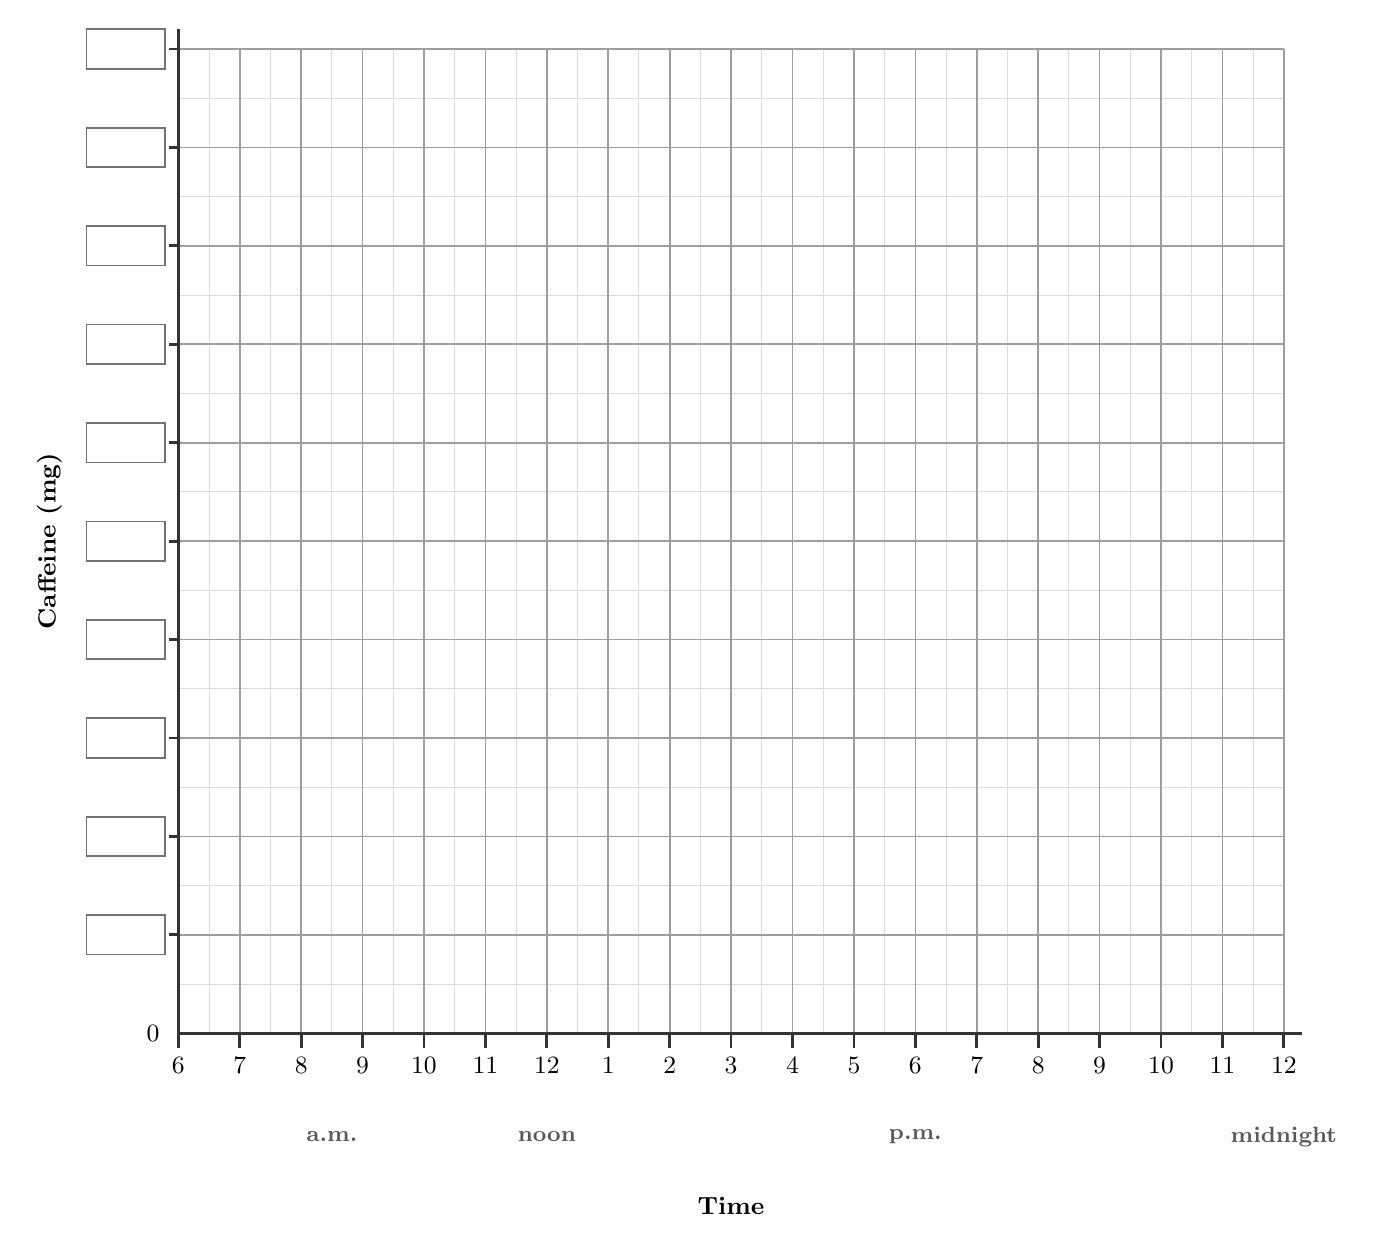
\begin{tikzpicture}[x=0.78cm, y=1.25cm]
    \draw[black!14, line width=0.35pt] (0,0) grid[xstep=0.5, ystep=0.5] (18,10);
    \draw[black!38, line width=0.6pt] (0,0) grid[xstep=1, ystep=1] (18,10);
    \draw[black!80, line width=1.2pt] (0,0) -- (0,10.2);
    \draw[black!80, line width=1.2pt] (0,0) -- (18.3,0);
    \node[left, font=\small] at (-0.15,0) {0};
    \foreach \v in {1,...,10}{
      \draw[black!80, line width=1pt] (0,\v) -- (-0.15,\v);
      \node[draw=black!55, line width=0.6pt, minimum width=1.0cm,
            minimum height=0.5cm, anchor=east, fill=white] at (-0.2,\v) {};}
    \foreach \h/\lab in {0/6,1/7,2/8,3/9,4/10,5/11,6/12,7/1,8/2,9/3,10/4,11/5,
                         12/6,13/7,14/8,15/9,16/10,17/11,18/12}{
      \draw[black!80, line width=1pt] (\h,0) -- (\h,-0.15);
      \node[below, font=\small] at (\h,-0.15) {\lab};}
    \node[font=\footnotesize\bfseries, text=black!65] at (2.5,-1.05) {a.m.};
    \node[font=\footnotesize\bfseries, text=black!65] at (6,-1.05) {noon};
    \node[font=\footnotesize\bfseries, text=black!65] at (12,-1.05) {p.m.};
    \node[font=\footnotesize\bfseries, text=black!65] at (18,-1.05) {midnight};
    \node[font=\small\bfseries] at (9,-1.75) {Time};
    \node[rotate=90, font=\small\bfseries] at (-2.1,5) {Caffeine (mg)};
  \end{tikzpicture}}

% ---------------------------------------------------------------------------
% HALF OF THE C3 TABLE. Two of these sit side by side, so twenty hours fit
% in half a page. #1 is the label above it.
% ---------------------------------------------------------------------------
\newcommand{\hourhalf}[1]{%
  {\small\bfseries\color{cbteal}#1}\par\vspace{3pt}
  {\setlength{\tabcolsep}{3pt}%
  \begin{tabular}{|C{1.55cm}|C{2.15cm}|C{1.55cm}|C{1.75cm}|}
    \hline
    \hrow \small\textbf{Time} & \small\textbf{Last hour}\newline$\times\,0.87$ &
      \small\textbf{$+$ Drink} & \small\textbf{Now}\newline\textbf{(mg)} \\ \hline
    \tall & & & \\ \hline
    \tall & & & \\ \hline
    \tall & & & \\ \hline
    \tall & & & \\ \hline
    \tall & & & \\ \hline
    \tall & & & \\ \hline
    \tall & & & \\ \hline
    \tall & & & \\ \hline
    \tall & & & \\ \hline
    \tall & & & \\ \hline
  \end{tabular}}}

\begin{document}

% ===========================================================================
% COVER
% ===========================================================================
\thispagestyle{fancy}

\begin{tcolorbox}[enhanced, colback=cbpurple!7, colframe=cbpurple!7, arc=7pt,
                  borderline west={6pt}{0pt}{cbpurple},
                  left=16pt, right=12pt, top=9pt, bottom=9pt]
  \begin{minipage}[c]{0.80\linewidth}
    {\color{cbpurple}\bfseries YEAR 7\sep SCIENCE\sep MODELS\sep CHALLENGE
    HOMEWORK}\\[5pt]
    {\color{cbpurple}\huge\bfseries Why Is Mr Bowen Still Awake?}\\[6pt]
    {\color{black!70}Half-life with real coffee, a real interview, and carbon
    dating}
  \end{minipage}\hfill
  \begin{minipage}[c]{0.15\linewidth}\centering
    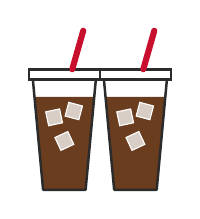
\begin{tikzpicture}[scale=0.95]
      \pic at (0,0) {coldbrew};
      \pic at (0.95,0) {coldbrew};
    \end{tikzpicture}
  \end{minipage}
\end{tcolorbox}

\vspace{4pt}
\noindent
\begin{tabularx}{\textwidth}{@{}X X@{}}
  \textbf{Name:} \blank[5.6cm] & \textbf{Class:} \blank[5.6cm] \\
  \textbf{Date given:} \blank[4.6cm] & \textbf{Date due:} \blank[4.8cm] \\
\end{tabularx}

\begin{activity}[How to do this homework]
  \begin{itemize}[itemsep=2pt, topsep=0pt]
    \item \textbf{Parts A and B:} Mr Bowen's coffee. They teach you the method.
    \item \textbf{Part C is the main task.} You interview an adult in your
      family. \textbf{Do the interview at the weekend.}
    \item \textbf{Part D:} carbon dating.
    \item You need a \textbf{calculator}, a \textbf{ruler}, and a
      \textbf{computer or phone}. Answer in \textbf{full sentences}.
  \end{itemize}
\end{activity}

\begin{remember}
  \key{Half-life:} the time it takes for half of something to disappear.
  Caffeine's half-life is about \key{5 hours}.

  \vspace{3pt}
  \key{Carbon-14:} a rare kind of carbon that slowly breaks down into nitrogen.
  Its half-life is \key{5\,700 years}.

  \vspace{3pt}
  \key{Carbon dating:} finding the age of something that was once alive by
  measuring how much carbon-14 is left. It only works for things that were
  \key{alive}, up to about \key{50\,000 years} old.
\end{remember}

% ===========================================================================
% PART A -- MR BOWEN'S REAL DAY
% ===========================================================================
\hwsection{Part A\quad Mr Bowen's Real Day}

\noindent This is what Mr Bowen really drinks on a school day.

\vspace{4pt}
\begin{center}
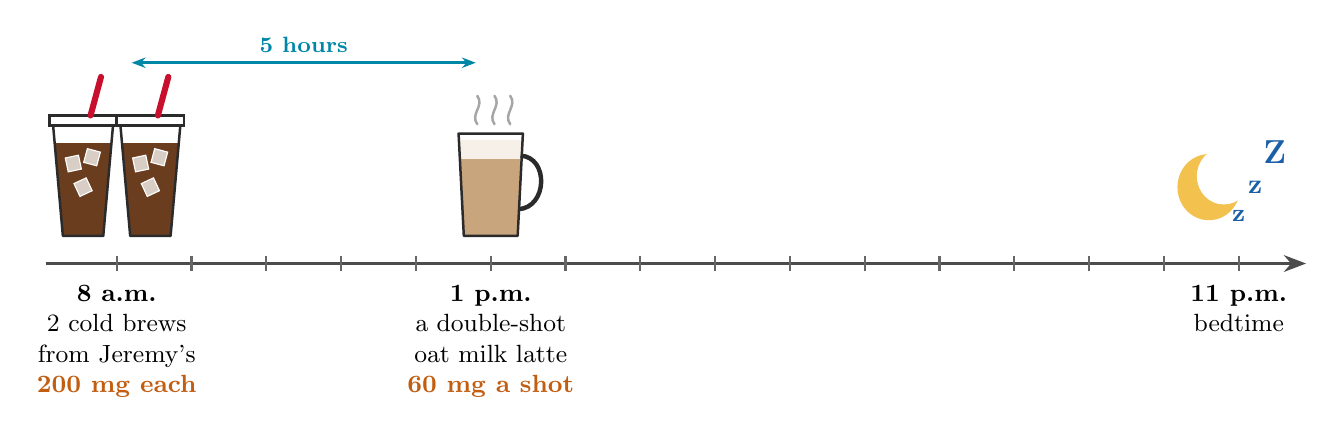
\begin{tikzpicture}[x=0.95cm, y=1cm]
  \draw[black!70, line width=1.4pt, -{Stealth[length=8pt]}] (-0.95,0) -- (15.9,0);
  \foreach \h in {0,...,15} \draw[black!60, line width=0.8pt] (\h,-0.1) -- (\h,0.1);
  % 8 a.m.
  \pic at (-0.45,0.35) {coldbrew};
  \pic at (0.45,0.35) {coldbrew};
  \node[below, align=center, font=\small] at (0,-0.15)
    {\textbf{8~a.m.}\\2 cold brews\\from Jeremy's\\
     {\color{cborange}\bfseries 200 mg each}};
  % 1 p.m.
  \pic at (5,0.35) {latte};
  \node[below, align=center, font=\small] at (5,-0.15)
    {\textbf{1~p.m.}\\a double-shot\\oat milk latte\\
     {\color{cborange}\bfseries 60 mg a shot}};
  % 11 p.m.
  \pic at (14.6,0.35) {bedtime};
  \node[below, align=center, font=\small] at (15,-0.15)
    {\textbf{11~p.m.}\\bedtime};
  % the gap
  \draw[cbteal, line width=0.9pt, {Stealth[length=5pt]}-{Stealth[length=5pt]}]
    (0.2,2.55) -- node[above, font=\footnotesize\bfseries, text=cbteal] {5 hours} (4.8,2.55);
\end{tikzpicture}
\end{center}

\begin{wordhelp}
  \renewcommand{\arraystretch}{1.15}
  \begin{tabularx}{\linewidth}{@{}W{2.9cm} L@{}}
    caffeine & a chemical in coffee, tea, cola and energy drinks. It keeps you
      awake. \\
    mg & milligram. $1\,000$ mg $= 1$ g. One grain of rice is about 20 mg. \\
    cold brew & strong coffee made slowly with cold water \\
    double shot & two shots. A \textbf{shot} is a small cup of very strong
      coffee. \\
    latte & coffee with a lot of milk. \textbf{Oat milk} is made from oats. \\
  \end{tabularx}
\end{wordhelp}

\qhead{A1}{The drinks}
\noindent (a) The cold brews: \ $2 \times 200 =$ \mg \hfill
(b) The latte: \ $2 \times 60 =$ \mg

\vspace{8pt}
\noindent (c) Does the \textbf{oat milk} add any caffeine?
\quad \tickbox\,\,yes \quad\; \tickbox\,\,no

\qhead{A2}{Half-life steps}
\noindent\begin{minipage}{\linewidth}
\noindent Fill in the boxes. Every 5 hours, \textbf{halve} (cut in half). When
he drinks, \textbf{add}.

\vspace{8pt}
\begin{center}
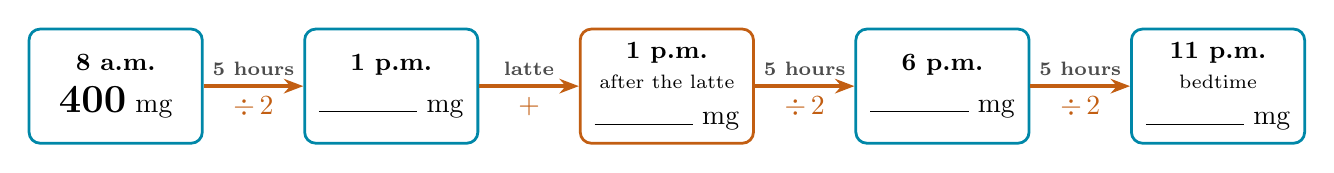
\begin{tikzpicture}[x=1cm, y=1cm]
  \node[cbox, minimum width=2.2cm] (a) at (0,0)
    {\textbf{\small 8~a.m.}\\[3pt]{\Large\bfseries 400} mg};
  \node[cbox, minimum width=2.2cm] (b) at (3.5,0)
    {\textbf{\small 1~p.m.}\\[3pt]\rule{1.25cm}{0.4pt} mg};
  \node[cbox, minimum width=2.2cm, draw=cborange] (c) at (7.0,0)
    {\textbf{\small 1~p.m.}\\[-1pt]{\scriptsize after the latte}\\[1pt]
     \rule{1.25cm}{0.4pt} mg};
  \node[cbox, minimum width=2.2cm] (d) at (10.5,0)
    {\textbf{\small 6~p.m.}\\[3pt]\rule{1.25cm}{0.4pt} mg};
  \node[cbox, minimum width=2.2cm] (e) at (14.0,0)
    {\textbf{\small 11~p.m.}\\[-1pt]{\scriptsize bedtime}\\[1pt]
     \rule{1.25cm}{0.4pt} mg};
  \draw[chainarrow] (a.east) -- node[above, font=\scriptsize\bfseries, text=black!70] {5 hours}
    node[below, font=\bfseries] {$\div\,2$} (b.west);
  \draw[chainarrow] (b.east) -- node[above, font=\scriptsize\bfseries, text=black!70] {latte}
    node[below, font=\bfseries] {$+$} (c.west);
  \draw[chainarrow] (c.east) -- node[above, font=\scriptsize\bfseries, text=black!70] {5 hours}
    node[below, font=\bfseries] {$\div\,2$} (d.west);
  \draw[chainarrow] (d.east) -- node[above, font=\scriptsize\bfseries, text=black!70] {5 hours}
    node[below, font=\bfseries] {$\div\,2$} (e.west);
\end{tikzpicture}
\end{center}
\end{minipage}

% ---------------------------------------------------------------------------
\qhead{A3}{Draw the graph}
\noindent\begin{minipage}{\linewidth}
\noindent Put a dot for every box in A2. The morning is drawn for you. At
1~p.m., draw a line \textbf{straight up}. Between the dots, draw a
\textbf{smooth curve}.

\vspace{6pt}
\begin{center}
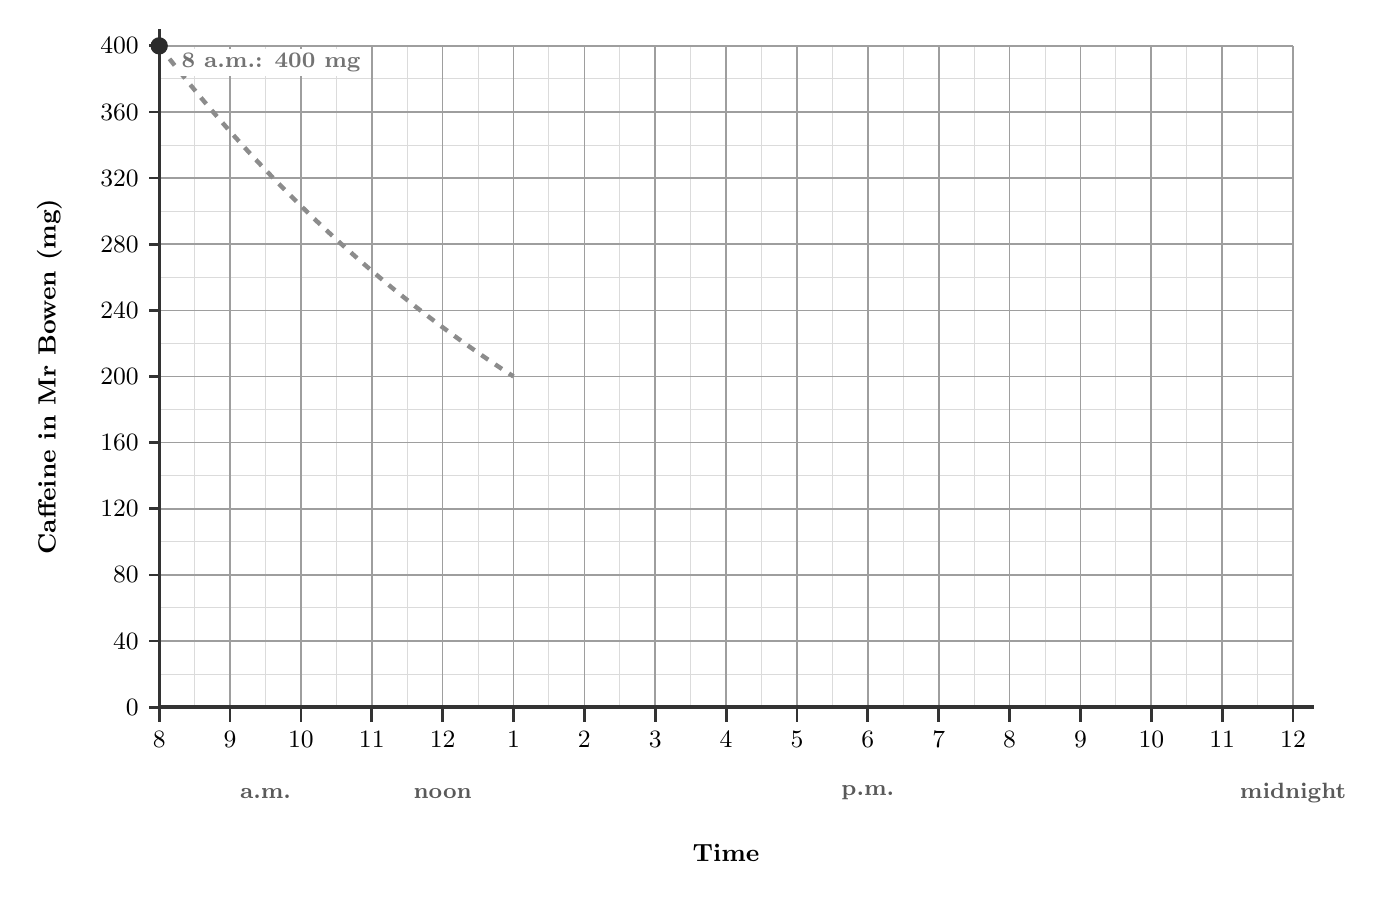
\begin{tikzpicture}[x=0.9cm, y=0.021cm]
  \bowenaxes
  \draw[black!45, line width=1.6pt, dashed] plot[domain=0:5, samples=40, smooth]
    (\x, {400*0.5^(\x/5)});
  \fill[ink] (0,400) circle (0.11cm);
  \node[right, font=\footnotesize\bfseries, text=black!55, fill=white,
        inner sep=1.5pt] at (0.25,390) {8~a.m.: 400 mg};
\end{tikzpicture}
\end{center}
\end{minipage}

\qhead{A4}{Read the graph}
\noindent (a) At 8~p.m. Mr Bowen is marking your homework. Go \textbf{up} from
8~p.m. to your curve, then \textbf{across}. How much caffeine is in him? \quad
\mg

\vspace{10pt}
\noindent (b) How much caffeine is in him at bedtime, 11~p.m.? \quad \mg

\vspace{10pt}
\noindent (c) Health experts say an adult should have \textbf{no more than
400 mg} of caffeine in a day. How much did Mr Bowen drink?

\vspace{4pt}
\noindent \blank[1.6cm] $+$ \blank[1.6cm] $=$ \mg \qquad Is that more than
400 mg? \blank[2.2cm]

\vspace{10pt}
\noindent (d) Tomorrow he wants \textbf{exactly 400 mg}. Which \textbf{one}
drink should he not buy?

\vspace{4pt}
\noindent He should not buy \blank[6.0cm]\,.

\qhead{A5}{The title question}
\noindent Why is Mr Bowen still awake at 11~p.m.? Use a number, and compare it
with a cup of coffee (about 100 mg).

\vspace{4pt}
\noindent\starter{At 11~p.m. Mr Bowen still has \ldots}
\qlines{3}

% ===========================================================================
% PART B -- HOUR BY HOUR
% ===========================================================================
\hwsection{Part B\quad Hour by Hour}

\begin{remember}[The hour-by-hour rule: it works for any time]
  \key{Every hour: $\times\,0.87$.} Round to a whole number.
  \qquad \key{When they drink: $+$ the drink.}

  \vspace{4pt}
  \noindent Example: Mr Bowen at 1~p.m. \quad $230 \times 0.87 = 200$, then
  $+\,120$ for the latte $= \mathbf{320}$ mg.
\end{remember}

\qhead{B1}{Why 0.87?}
\noindent\begin{minipage}{\linewidth}
\noindent Start with 100 mg. Multiply by 0.87 every hour. Round each answer.

\vspace{8pt}
\begin{center}
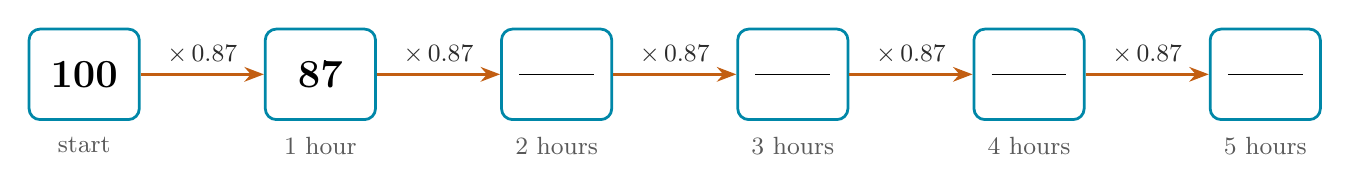
\begin{tikzpicture}[x=1cm, y=1cm]
  \tikzset{nbox/.style={cbox, minimum width=1.4cm, minimum height=1.15cm}}
  \node[nbox] (n0) at (0,0)    {\Large\bfseries 100};
  \node[nbox] (n1) at (3.0,0)  {\Large\bfseries 87};
  \node[nbox] (n2) at (6.0,0)  {\rule{0.95cm}{0.4pt}};
  \node[nbox] (n3) at (9.0,0)  {\rule{0.95cm}{0.4pt}};
  \node[nbox] (n4) at (12.0,0) {\rule{0.95cm}{0.4pt}};
  \node[nbox] (n5) at (15.0,0) {\rule{0.95cm}{0.4pt}};
  \foreach \i/\lab in {0/start, 1/1 hour, 2/2 hours, 3/3 hours, 4/4 hours,
                       5/5 hours}
    \node[below, font=\small, text=black!65] at (\i*3.0,-0.68) {\lab};
  \foreach \i [evaluate=\i as \j using int(\i+1)] in {0,...,4}
    \draw[chainarrow] (n\i.east) -- node[above, font=\small\bfseries, text=ink]
      {$\times\,0.87$} (n\j.west);
\end{tikzpicture}
\end{center}

\vspace{2pt}
\noindent After 5 hours, about how much is left? \blank[3.0cm] \quad That is
one \blank[3.0cm]\,.
\end{minipage}

\qhead{B2}{Check it with Mr Bowen}
\noindent\begin{minipage}{\linewidth}
\noindent Use the rule from 1~p.m. to 8~p.m. (He drinks nothing in this time.)

\vspace{6pt}
\noindent\begin{tabular}{|C{1.47cm}|C{1.47cm}|C{1.47cm}|C{1.47cm}|C{1.47cm}|C{1.47cm}|C{1.47cm}|C{1.47cm}|}
  \hline
  \hrow 1~p.m. & 2~p.m. & 3~p.m. & 4~p.m. & 5~p.m. & 6~p.m. & 7~p.m. & 8~p.m. \\ \hline
  \starter{320}\tall & & & & & & & \\ \hline
\end{tabular}

\vspace{8pt}
\noindent Is your 6~p.m. number about the same as in A2? \hfill
\tickbox\,\,yes \quad\; \tickbox\,\,no

\vspace{4pt}
\noindent Is your 8~p.m. number about the same as in A4(a)? \hfill
\tickbox\,\,yes \quad\; \tickbox\,\,no

\vspace{8pt}
\noindent When different methods agree, scientists \blank[3.0cm] the answer.
\end{minipage}

% ===========================================================================
% PART C -- THE MAIN TASK
% ===========================================================================
\hwsection{Part C\quad Interview a Caffeine Drinker \hfill \maintag}

\begin{activity}[What you will do]
  \noindent \textbf{Interview} an adult in your family who drinks caffeine:
  a parent, a grandparent, an aunt, an uncle. Ask about coffee, tea, soda
  (like Coca-Cola) or \textbf{energy drinks like Sting}. Then
  \textbf{estimate} how much caffeine is in their body at bedtime.

  \vspace{4pt}
  \noindent Nobody at home drinks caffeine? Ask another adult you know. You can
  do the interview in \textbf{any language}. Write in \textbf{English}.
\end{activity}

\qhead{C1}{The interview}
\noindent Ask about \textbf{yesterday}, or another normal day.

\begin{multicols}{2}
\begin{enumerate}[label=\textbf{\arabic*.}, itemsep=2pt, topsep=2pt]
  \item ``Can I interview you for my homework?''
  \item ``What did you drink that has caffeine?''
  \item ``What time did you drink it?''
  \item ``How big was it? A cup, a can, a bottle?''
  \item ``What brand was it?''
  \item ``What time did you go to bed?''
\end{enumerate}
\end{multicols}

\vspace{2pt}
\noindent\textbf{I interviewed my} \blank[4.0cm]\,. \qquad
\textbf{They went to bed at} \blank[3.0cm]\,.

\vspace{8pt}
\noindent\begin{minipage}{\linewidth}
\noindent Write their drinks here. Round each time to the \textbf{nearest hour}:
7:40 $\rightarrow$ 8:00, \ 10:20 $\rightarrow$ 10:00. Fill in the last two
columns in C2.

\vspace{6pt}
\renewcommand{\arraystretch}{1.2}
\noindent\begin{tabularx}{\linewidth}{|L|C{1.75cm}|C{1.75cm}|C{1.75cm}|C{3.3cm}|}
  \hline
  \hrow \textbf{Drink}\newline{\small what, and how big} & \textbf{Time} &
    \textbf{Rounded time} & \textbf{Caffeine}\newline\textbf{(mg)} &
    \textbf{Where I found it} \\ \hline
  \starter{\small \textit{Example:} 1 can of cola, 330 ml} &
    \starter{\small 3:40 p.m.} & \starter{\small 4~p.m.} & \starter{\small 32} &
    \starter{\small the company's website} \\ \hline
  \tall & & & & \\ \hline
  \tall & & & & \\ \hline
  \tall & & & & \\ \hline
  \tall & & & & \\ \hline
\end{tabularx}
\end{minipage}

% ---------------------------------------------------------------------------
\qhead{C2}{Find the caffeine}

\begin{activity}[Where to look]
  \begin{minipage}[t]{0.68\linewidth}
    \begin{enumerate}[label=\textbf{\arabic*.}, itemsep=3pt, topsep=0pt]
      \item \textbf{The label} on the can or bottle. Look for the word
        \textbf{caffeine}. It often says how many mg are in \textbf{100 ml}.
      \item \textbf{The company's website.}
      \item \textbf{Search:} \textit{caffeine in [the drink] mg}, for example
        \textit{caffeine in Sting 330 ml}.
    \end{enumerate}

    \vspace{5pt}
    \noindent Milk, sugar, ice and condensed milk: \key{0 mg}.

    \vspace{3pt}
    \noindent Two numbers, like 50 to 80 mg? Use the \textbf{middle}: 65 mg.
  \end{minipage}\hfill
  \begin{minipage}[t]{0.28\linewidth}\vspace{-6pt}\centering
    % A bottle with its label. No real brand: the numbers are made up.
    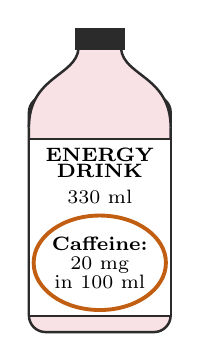
\begin{tikzpicture}[x=1cm, y=1cm]
      \draw[ink, line width=0.9pt, fill=cbred!12, rounded corners=6pt]
        (-0.9,0) rectangle (0.9,3.0);
      \draw[ink, line width=0.9pt, fill=cbred!12]
        (-0.9,2.6) .. controls (-0.9,3.25) and (-0.3,3.25) .. (-0.27,3.6) --
        (0.27,3.6) .. controls (0.3,3.25) and (0.9,3.25) .. (0.9,2.6);
      \draw[ink, line width=0.9pt, fill=ink] (-0.3,3.6) rectangle (0.3,3.85);
      \draw[ink, line width=0.6pt, fill=white] (-0.9,0.2) rectangle (0.9,2.45);
      \node[font=\scriptsize\bfseries, align=center] at (0,2.15) {ENERGY\\[-2pt]DRINK};
      \node[font=\scriptsize] at (0,1.72) {330 ml};
      \node[font=\scriptsize, align=center] at (0,0.88)
        {\textbf{Caffeine:}\\[-1pt]20 mg\\[-1pt]in 100 ml};
      \draw[cborange, line width=1.4pt] (0,0.88) ellipse (0.84cm and 0.6cm);
    \end{tikzpicture}
  \end{minipage}
\end{activity}

\noindent\begin{minipage}{\linewidth}
\noindent\textbf{Reading a label.} This bottle has 20 mg in every 100 ml. It
holds 330 ml.

\vspace{3pt}
\noindent $330 \div 100 = 3.3$ \qquad $3.3 \times 20 = $ \key{66 mg} in the
whole bottle.

\vspace{10pt}
\noindent (a) \textbf{10 mg in 100 ml}, a \textbf{330 ml} can: \quad
\blank[1.5cm] $\times\ 10 =$ \mg

\vspace{10pt}
\noindent (b) \textbf{30 mg in 100 ml}, a \textbf{250 ml} can: \quad
\blank[1.5cm] $\times\ 30 =$ \mg

\vspace{10pt}
\noindent Now look up every drink in C1. Fill in the \textbf{Caffeine} and
\textbf{Where I found it} columns.
\end{minipage}

% ---------------------------------------------------------------------------
\qhead{C3}{Hour by hour}
\noindent\begin{minipage}{\linewidth}
\noindent Use the rule from Part B and the \textbf{rounded} times. Row 1 is
their \textbf{first} drink. Each row is \textbf{one hour later}. Stop at
\textbf{bedtime}.

\vspace{8pt}
\noindent\begin{minipage}[t]{0.49\linewidth}\centering
  \hourhalf{Start here}
\end{minipage}\hfill
\begin{minipage}[t]{0.49\linewidth}\centering
  \hourhalf{Then carry on here}
\end{minipage}
\end{minipage}

% ---------------------------------------------------------------------------
\qhead{C4}{Draw their graph}
\noindent\begin{minipage}{\linewidth}
\noindent\textbf{Step 1.} Find the biggest number in your table. Choose one
big square from this table, and write the numbers in the boxes on the graph.

\vspace{6pt}
\begin{center}
\renewcommand{\arraystretch}{1.25}
\begin{tabular}{|l|C{1.5cm}|C{1.5cm}|C{1.5cm}|C{1.5cm}|C{1.5cm}|}
  \hline
  \hrow \textbf{Biggest number} & under 100 & under 200 & under 300 &
    under 400 & under 600 \\ \hline
  \textbf{One big square} $=$ & 10 mg & 20 mg & 30 mg & 40 mg & 60 mg \\ \hline
\end{tabular}
\end{center}

\vspace{4pt}
\noindent\textbf{Step 2.} Put a dot for every row of your table. At a drink, go
\textbf{straight up}. Between the dots, draw a \textbf{smooth curve}.

\vspace{6pt}
\begin{center}
\mygraph
\end{center}
\end{minipage}

% ---------------------------------------------------------------------------
% Page 7 is the results and the check; page 8 is Part D on its own. Forced
% breaks, because each of the last three pages is one job.
\clearpage
\qhead{C5}{Your results}
\noindent (a) At bedtime (\blank[1.6cm]), my \blank[2.6cm] had about
\blank[1.6cm] mg of caffeine in their body.

\vspace{12pt}
\noindent (b) Compare with Mr Bowen (80 mg at bedtime).

\vspace{2pt}
\noindent\starter{My \blank[2.4cm] had more / less caffeine at bedtime than
Mr Bowen, because \ldots}
\qlines{3}

\vspace{6pt}
\noindent\begin{minipage}{\linewidth}
\noindent (c) \textbf{Challenge.} They want less caffeine at bedtime. Give them
\textbf{one} piece of advice. Use a number from your table.

\vspace{2pt}
\noindent\starter{I think they should \ldots\ because \ldots}
\wlines{3}
\end{minipage}

\vspace{10pt}
\noindent\begin{minipage}{\linewidth}
\noindent (d) Your model is an estimate. Give \textbf{one} reason your bedtime
number might be wrong. \textit{Clue:} caffeine's half-life is not 5 hours for
everybody. It can be from about 1.5 to 9.5 hours.

\vspace{2pt}
\noindent\starter{My bedtime number might be wrong because \ldots}
\wlines{3}
\end{minipage}

\begin{yourturn}[Before you hand it in: tick each one]
  \renewcommand{\arraystretch}{1.75}
  \begin{tabularx}{\linewidth}{@{}p{0.8cm}L@{}}
    \tickbox & Every drink in C1 has a time, the caffeine in mg, and where I
      found it. \\
    \tickbox & My C3 table goes up \textbf{one hour} a row and stops at
      bedtime. \\
    \tickbox & Each drink is added \textbf{once}, in its own hour. \\
    \tickbox & My graph goes \textbf{straight up} at every drink. \\
    \tickbox & My bedtime number is the \textbf{same} in C3, C4 and C5(a). \\
  \end{tabularx}
\end{yourturn}

% ===========================================================================
% PART D -- CARBON DATING
% ===========================================================================
\clearpage
\hwsection{Part D\quad Carbon Dating}
\qhead{D1}{The halving chain}
\noindent\begin{minipage}{\linewidth}
\noindent Caffeine halves every 5 hours. Carbon-14 halves every
\textbf{5\,700 years}. Fill in the boxes.

\vspace{8pt}
\begin{center}
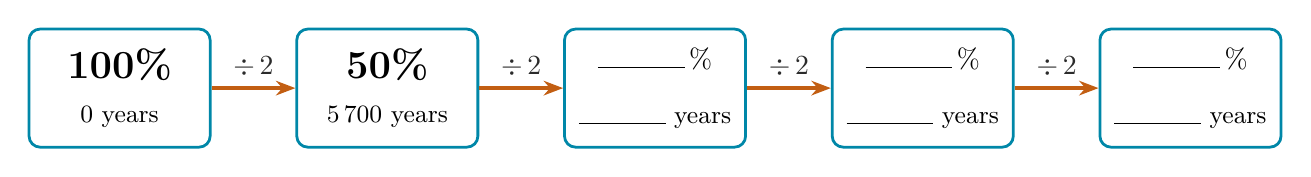
\begin{tikzpicture}[x=1cm, y=1cm]
  \tikzset{kbox/.style={cbox, minimum width=2.3cm, minimum height=1.5cm}}
  \node[kbox] (k0) at (0,0)    {{\Large\bfseries 100\%}\\[4pt]{\small 0 years}};
  \node[kbox] (k1) at (3.4,0)  {{\Large\bfseries 50\%}\\[4pt]{\small 5\,700 years}};
  \node[kbox] (k2) at (6.8,0)  {\rule{1.1cm}{0.4pt}\,\%\\[8pt]{\small\rule{1.1cm}{0.4pt} years}};
  \node[kbox] (k3) at (10.2,0) {\rule{1.1cm}{0.4pt}\,\%\\[8pt]{\small\rule{1.1cm}{0.4pt} years}};
  \node[kbox] (k4) at (13.6,0) {\rule{1.1cm}{0.4pt}\,\%\\[8pt]{\small\rule{1.1cm}{0.4pt} years}};
  \foreach \i [evaluate=\i as \j using int(\i+1)] in {0,...,3}
    \draw[chainarrow] (k\i.east) -- node[above, font=\bfseries, text=ink]
      {$\div\,2$} (k\j.west);
\end{tikzpicture}
\end{center}
\end{minipage}

% ---------------------------------------------------------------------------
\qhead{D2}{The museum}
\noindent\begin{minipage}{\linewidth}
\noindent Scientists measured the carbon-14 left in six objects. Use D1.
\textbf{Careful:} carbon dating does not work for everything.

\vspace{6pt}
\renewcommand{\arraystretch}{1.2}
\noindent\begin{tabularx}{\linewidth}{|L|C{2.2cm}|C{2.2cm}|C{2.2cm}|C{2.8cm}|}
  \hline
  \hrow \textbf{Object} & \textbf{Was it ever alive?} & \textbf{Carbon-14
    left} & \textbf{How many half-lives?} & \textbf{Age (years)} \\ \hline
  \starter{A wooden boat from a river}\tall & \starter{yes} & \starter{50\%} &
    \starter{1} & \starter{5\,700} \\ \hline
  A bear bone from a cave\tall & & 12.5\% & & \\ \hline
  Charcoal {\small(burnt wood)}\tall & & 6.25\% & & \\ \hline
  A cotton T-shirt, made this year\tall & & 100\% & & \\ \hline
  A stone axe\tall & & --- & & \\ \hline
  A \textit{Tyrannosaurus rex} tooth\tall & & 0\% & & \\ \hline
\end{tabularx}

\vspace{3pt}
\noindent{\small\color{cbblue}\textbf{Word help:} \textbf{cotton} comes from a
plant \sep an \textbf{axe} is a tool for cutting wood}
\end{minipage}

% ---------------------------------------------------------------------------
\qhead{D3}{Same model, different clock}
\noindent While Mr Bowen is alive, \textbf{coffee} tops up his caffeine and
\textbf{food} tops up his carbon-14. What is the \textbf{same} about caffeine
and carbon-14? What is \textbf{different}? Use the word \textbf{half-life}.

\vspace{4pt}
\noindent\starter{They are the same because \ldots\ The difference is \ldots}
\qlines{5}

% ===========================================================================
% ANSWER KEY -- TEACHER COPY ONLY
% ===========================================================================
\ifkey
\clearpage

\hwsection[cbred]{Answer Key --- Teacher Copy}

\linespread{1.0}\selectfont
\setlist[enumerate]{itemsep=2pt, topsep=3pt, leftmargin=*}
\setlist[itemize]{itemsep=2pt, topsep=3pt, leftmargin=*}

\noindent{\small Mr Bowen's numbers are chosen so Part A is exact: the drinks
are 5 hours apart and bed is 10 hours after the latte. The rule in Part B rounds
at every step and lands within 1 mg of Part A. Accept $\pm 3$ mg anywhere from a
student who rounded at a different step.}

\qhead[cbred]{A1}{The drinks}
\noindent (a) \textbf{400} mg \sep (b) \textbf{120} mg \sep (c) \textbf{no}

\smallskip
\noindent{\small Expect 60 for (b) from a student who read \emph{double-shot}
as one shot. (c) is there for Part C: the condensed milk in a Vietnamese iced
coffee adds nothing either, and a student who counts the whole drink will not
know which number to look up.}

\qhead[cbred]{A2}{Half-life steps}
\noindent 1~p.m.: \textbf{200} \sep after the latte: \textbf{320} \sep 6~p.m.:
\textbf{160} \sep 11~p.m.: \textbf{80}

\smallskip
\noindent{\small \textbf{The latte box is the question.} Expect 100 and 50 from
a student who halved straight through it, and 260 / 130 / 65 from one who
added 60. If the second box is 520, they added the latte to the 8~a.m. number
before halving --- ask what happened between 8~a.m. and 1~p.m.}

\qhead[cbred]{A3}{The graph}
\begin{center}
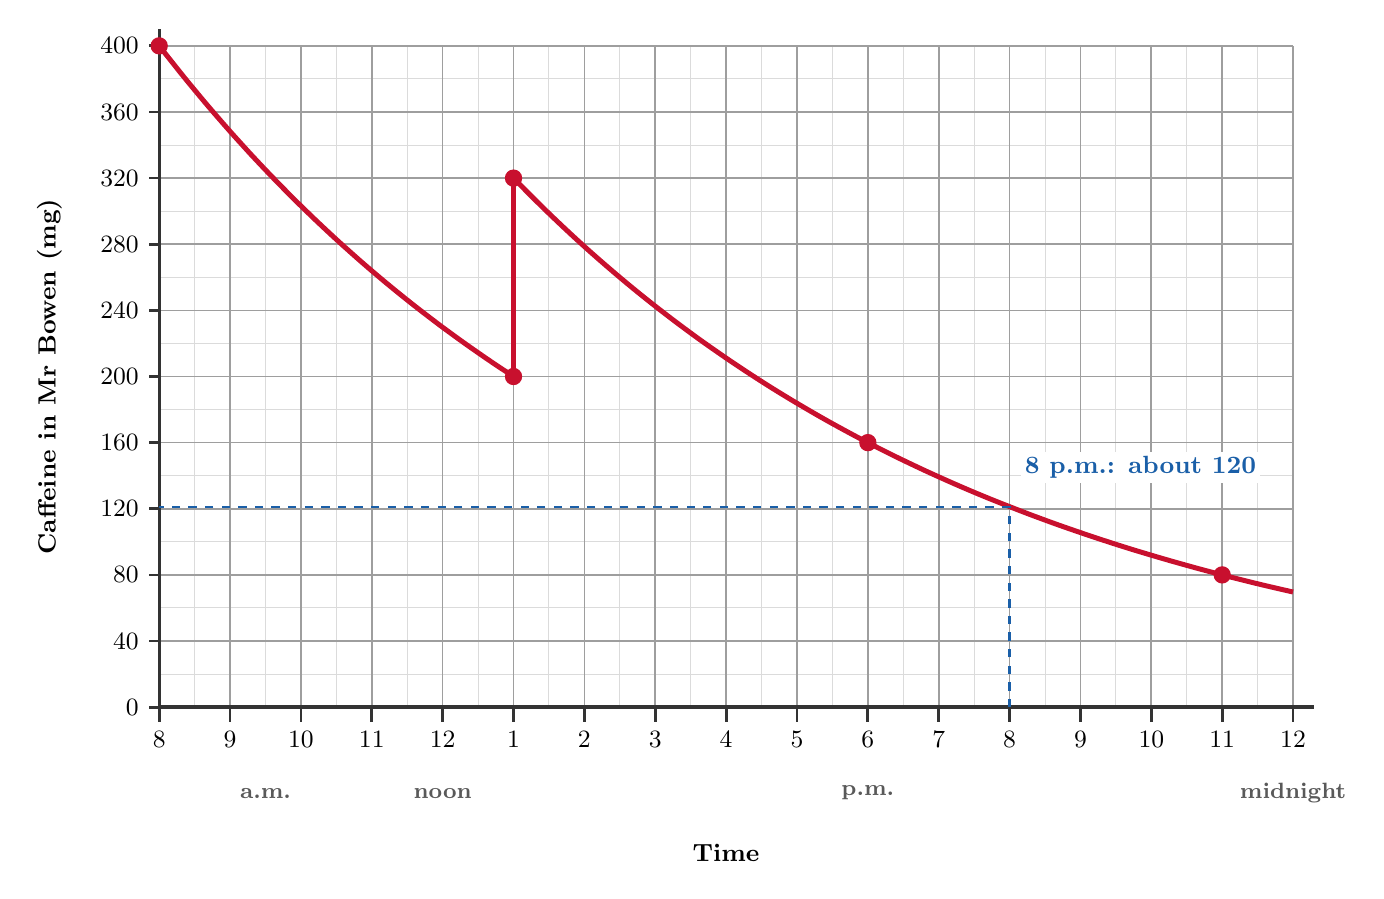
\begin{tikzpicture}[x=0.9cm, y=0.021cm]
  \bowenaxes
  \draw[cbred, line width=1.8pt] plot[domain=0:5, samples=40, smooth]
    (\x, {400*0.5^(\x/5)});
  \draw[cbred, line width=1.8pt] (5,200) -- (5,320);
  \draw[cbred, line width=1.8pt] plot[domain=5:16, samples=60, smooth]
    (\x, {320*0.5^((\x-5)/5)});
  \foreach \h/\v in {0/400, 5/200, 5/320, 10/160, 15/80}
    \fill[cbred] (\h,\v) circle (0.11cm);
  \draw[cbblue, line width=1pt, dashed] (12,0) -- (12,121) -- (0,121);
  \node[right, font=\small\bfseries, text=cbblue, fill=white, inner sep=1.5pt]
    at (12.15,145) {8~p.m.: about 120};
\end{tikzpicture}
\end{center}

\noindent{\small Look for the \textbf{vertical} jump at 1~p.m. A slope from
noon to 1~p.m. means the student is joining dots, not modelling a drink. Two
straight lines instead of curves is the other common one; it makes A4(a) come
out at 128 instead of 121.}

\qhead[cbred]{A4}{Read the graph}
\noindent (a) about \textbf{120} mg (exactly 121; accept 115--130) \sep (b)
\textbf{80} mg \\
(c) $400 + 120 = \mathbf{520}$ mg; \textbf{yes} \sep (d) \textbf{the latte}
($520 - 120 = 400$)

\smallskip
\noindent{\small (d): ``one cold brew'' gives 320, which is under 400 but not
\emph{exactly} 400 --- worth a minute in class, because both are healthier and
only one answers the question asked.}

\qhead[cbred]{A5}{The title question}
\noindent\textit{At 11~p.m. Mr Bowen still has 80 mg of caffeine in his body.
That is almost a whole cup of coffee.}

\smallskip
\noindent{\small Check for the number \emph{and} the comparison. ``Because he
drank coffee'' is true and is not the answer.}

\qhead[cbred]{B1}{Why 0.87?}
\noindent 100, 87, \textbf{76, 66, 57, 50} \sep about \textbf{50 mg}, which is
\textbf{half}: one \textbf{half-life} \quad ($0.87^5 = 0.498$)

\qhead[cbred]{B2}{Check it with Mr Bowen}
\noindent 320, \textbf{278, 242, 211, 184, 160, 139, 121} \sep yes, yes \sep
scientists \textbf{trust} the answer

\smallskip
\noindent{\small The last line is deck slide 43, word for word. Expect 160, 80,
40, 20 \ldots\ from a student who halved every hour instead of
$\times\,0.87$ (both of B2's checks then come out ``no''): that is the error to catch
before Part C, where it would put every family member at almost zero by
bedtime.}

\qhead[cbred]{C1--C4}{The interview, the table, the graph}
\noindent{\small No single answer. Mark in this order, and stop at the first
thing that is missing --- it is the thing to send back:}
\begin{enumerate}
  \item A real person, named by relationship (``my father''), with a bedtime.
  \item Every drink has a time, a rounded time, an amount in mg, and
    \textbf{where the number came from}. ``Google'' is acceptable; a blank is
    not.
  \item C2: (a) $3.3 \times 10 = \mathbf{33}$ mg \sep (b) $2.5 \times 30 =
    \mathbf{75}$ mg.
  \item C3 starts at the first drink, goes up one hour a row (left table, then
    right), and stops at bedtime. Each row is the row above $\times\,0.87$; a
    drink appears \emph{once}, in its own row.
  \item C4: the scale goes up in equal steps from the table, the dots match C3,
    drinks are vertical jumps, and the bedtime value on the graph is the last
    row of C3.
\end{enumerate}

\noindent{\small \textbf{Numbers to sanity-check against} (all approximate; the
point is that the student found one and said where): Sting, 330 ml bottle,
about 50--85 mg (the Vietnamese label gives a range per litre, which is a good
C2 conversation) \sep cola, 330 ml can, about 30--35 mg \sep Red Bull, 250 ml
can, about 50--80 mg depending on the version \sep one espresso shot, about
60--75 mg \sep Vietnamese iced coffee, about 100--200 mg (robusta, and very
variable) \sep a cup of black or green tea, about 30--50 mg.}

\smallskip
\noindent{\small \textbf{Expect at least one sheet where bedtime is above Mr
Bowen's 80 mg.} An afternoon iced coffee and an evening Sting will do it. That
sheet is worth showing the class (without the name).}

\qhead[cbred]{C5}{Results}
\noindent{\small (a) must match the last row of C3. (b) needs \emph{because}
and a reason from the table: more drinks, a bigger drink, or a later drink.
(c) the strongest advice moves or cuts the \textbf{last} drink of the day ---
an afternoon drink matters far more at bedtime than a morning one. Credit a
student who reworks the table to show it. (d) accept: the half-life is
different for different people (the clue); the caffeine numbers are estimates
and brands differ; times were rounded; the person may not remember exactly;
the model adds a drink all at once, but caffeine takes time to get into the
blood; yesterday may not have been a normal day. ``I might have made a
mistake'' is not a limitation of the model --- ask which part of the model.}

\qhead[cbred]{D1}{The halving chain}
\noindent 100\%, 50\%, \textbf{25\%, 12.5\%, 6.25\%} \sep 0, 5\,700,
\textbf{11\,400, 17\,100, 22\,800} years

\qhead[cbred]{D2}{The museum}
\renewcommand{\arraystretch}{1.2}
\noindent\begin{tabularx}{\linewidth}{@{}p{2.8cm}>{\raggedright\arraybackslash}p{4.4cm}p{1.3cm}p{0.5cm}L@{}}
  bear bone & yes & 12.5\% & 3 & \textbf{17\,100} \\
  charcoal & \textbf{yes} (it was wood) & 6.25\% & 4 & \textbf{22\,800} \\
  cotton T-shirt & \textbf{yes} (cotton is a plant) & 100\% & 0 &
    \textbf{about 0} (it is new) \\
  stone axe & \textbf{no} & --- & --- & carbon dating does not work \\
  \textit{T.\ rex} tooth & yes & 0\% & --- & too old: over 50\,000 years \\
\end{tabularx}

\smallskip
\noindent{\small \textbf{The three traps are the question.} Expect ``no'' for
charcoal and the T-shirt from students who read \emph{alive} as \emph{an
animal}. Expect ``no'' for the \textit{T.\ rex} because it is dead --- it was
alive; it is too old (deck slide 31: 66 million years, over 11\,000
half-lives). A student who writes ``date the volcanic ash'' has remembered
slide 34; give credit.}

\qhead[cbred]{D3}{Same model, different clock}
\noindent\textit{They are the same because both get topped up while he is
alive, and when the top-ups stop, both halve every half-life. The difference
is the half-life: 5 hours for caffeine and 5\,700 years for carbon-14.}

\smallskip
\noindent{\small Deck slide 25: ``food and drink keep topping up your
carbon-14. Even coffee.'' A student who says only ``they both halve'' has the
first half; push for the difference in the clock.}

\fi

\end{document}
